%!TeX root=../index.tex

\section{Einleitung}\label{sec:introduction}

Der folgende Text dient der Dokumentation eines Programmierprojekts, welches im Rahmen der Vorlesung \texttt{TM40401.1 Mobile Computing} durchgeführt wurde.
Es galt mittels des Frameworks \emph{flutter}\footnote{\url{https://flutter.dev/}} eine Mobile-App zu entwickeln, welche Kindern (im Alter von ca. 6--8) das kleine Einmaleins beizubringen.
Der Quellcode der App ist auf GitHub zu finden: \url{https://github.com/kevinsieverding/dhbw-tm404011-app}.

Diese Dokumentation beschreibt zunächst den Prozess wie das grundlegende Konzept für die App hergeleitet wurde.
Anschließend wird die App im Detail betrachtet, bevor der Schluss die Inhalten noch einmal kurz zusammenfasst und einen Ausblick über die möglichen Weiterentwicklungen bietet.

\section{Methode}

\subsection{Grundannahmen}

Abgeleitet von der Zielgruppe---Kinder im Alter von ca. 6--8 Jahren---habe ich zunächst einige Grundannahmen abgeleitet, was die Gestaltung der Lernfunktion angeht.
Kinder in diesem Alter haben nur eine kurze Aufmerksamkeitsspanne und können sich nur begrenzt selbst motivieren. Gleichzeitig haben sie allerdings auch eine große Neugier und einen ausgeprägten Spieltrieb.

Daher habe ich mich früh dazu entschieden Techniken der Gamification einzusetzen um den Lernprozess spielerisch zu gestalten.
Dies soll dazu beitragen, dass die Kinder länger aufmerksam bleiben und von sich aus mit der Applikation lernen möchten.

Eine---nicht zwingend ausführliche---Liste der Gamification-Techniken, welche ich in diesem Zusammenhang betrachtet habe sind:

\begin{itemize}
  \item Feedback
  
  Der Spielerin positives Feedback in Form von visuellen und/oder auditiven Effekten geben.

  Zum Beispiel, Konfetti anzeigen, wenn eine Höchstpunktzahl geknackt wurde. Eventuell zusammen mit einem Soundeffekt von jubelnden Kindern oder einer Partytröte.

  \item Punkte
  
  Dem Spieler ein positives Gefühl geben, indem er abstrakte Punkte für das Durchführen von bestimmten Handlungen erhält.

  Zum Beispiel, dem Spieler für jede korrekt gelöste Aufgabe zehn Punkte auf ein Konto gutschreiben und die Höchstpunktzahl festhalten und Anzeigen, um den Spieler dazu anzuspornen, sie zu übertreffen.

  \item Ranglisten
  
  Die Spielerin zum Wettkampf gegen andere Spieler oder sich selbst animieren, indem die eigene Punktzahl und die anderer Spieler in einer Rangliste angezeigt werden.

  \item Errungenschaften
  
  Den Spieler für das Erreichen bestimmter Meilensteine mit einer Errungenschaft belohnen.

  Zum Beispiel, dem Spieler für das Erreichen von 10.000 Punkten ein Abzeichen verleihen, welches er sich auf einer Profilansicht anzeigen lassen kann.

  \item Herausforderung
  
  Den Lernprozess für die Spielerin abwechslungsreicher gestalten, indem dem Prozess virtuelle Herausforderungen hinzugefügt werden.
  
  Zum Beispiel, durch das hinzufügen von Zeitlimits oder von Geschicklichkeitsprüfungen.
\end{itemize}

\subsection{Brainstorming}

Aufbauend auf diesen Grundannahmen bin ich in ein Brainstorming übergegangen, bei dem ich mich von mir bereits bekannten Spiel- und Lern-App-Ansätzen habe inspirieren lassen.
Als Ergebnis erhielt ich sechs vielversprechende Ansätze, von denen ich nur noch einen auswählen musste.

Im Folgenden möchte ich auf jeden Ansatz kurz eingehen und anschließend darlegen für welchen ich mich entschieden habe und warum.

\begin{enumerate}
  \item Dynamisches Richtig-Falsch-Spiel mit Tinder-Swipe-Mechanik
  
  \begin{figure}[h]
    \centering
    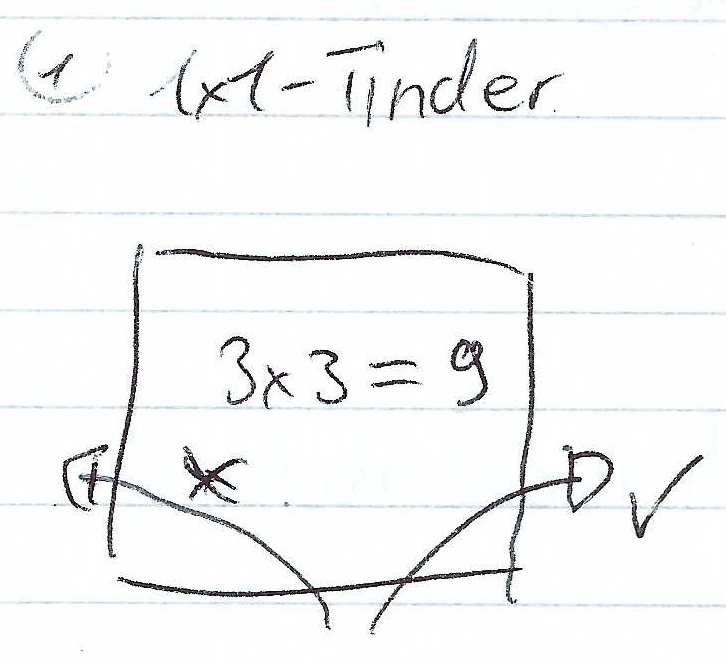
\includegraphics[width=0.5\textwidth]{brainstorming_01_tinder.png}
    \caption{Skizze des Tinder-Ansatzes}
  \end{figure}

  Beim ersten Ansatz soll die Spielerin zufällig generierte Gleichungen aus dem Einmaleins in richtig und falsch einordnen, indem sie die Karte auf der die Aufgabe steht entweder nach links oder rechts wischt.
  Während diese Mechanik vor allem von der Dating-App \emph{Tinder}\footnote{\url{https://tinder.com/}} bekannt ist, so hat das Videospiel \emph{REIGNS}\footnote{\url{https://reignsgame.com/reigns/}} sie bereits in einem Spiel-Kontext eingesetzt.

  \item Zum richtigen Ergebnis kommen mit viel Tippen unter Zeitdruck
  
  \begin{figure}[h]
    \centering
    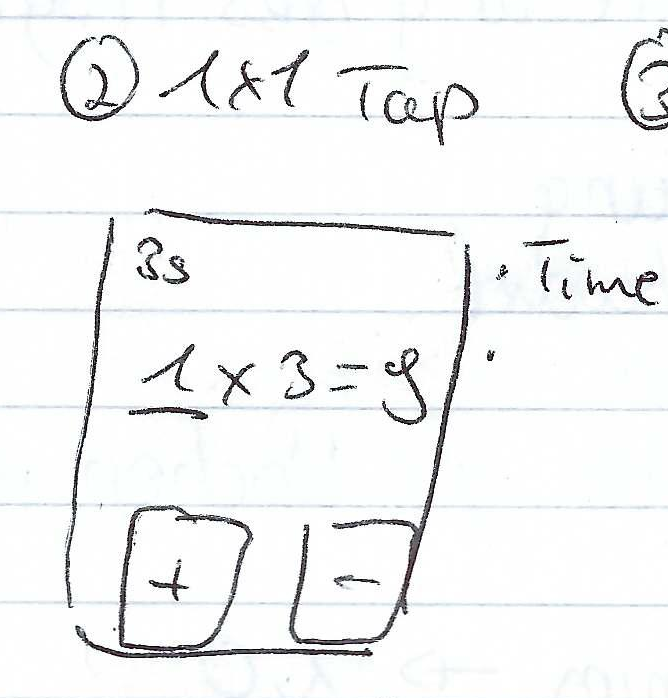
\includegraphics[width=0.5\textwidth]{brainstorming_02_tap.png}
    \caption{Skizze des Tipp-Ansatzes}
  \end{figure}

  Dieser Ansatz präsentiert dem Spieler eine Reihe von Gleichungen aus dem Einmaleins, welche immer ein falsches Ergebnis haben.
  Das Ergebnis kann mittels zweier Knöpfe in- oder dekrementiert werden um es zu korrigieren.
  Ein knapper Countdown soll die Aufgabe herausfordernder machen und den Spieler dazu verleiten in Eile über das Ziel hinauszuschießen.

  \item Rechenaufgaben in interessanten Verkleidungen
  
  Dieser Ansatz verkleidet Multiplikationsaufgaben in für Kinder ansprechendere Analogien, wie zum Beispiel das Mischen von Zutaten beim Kochen oder beim Brauen von Zaubertränken.

  \item Hexagon-Kombinationsspiel á la Dorfromantik
  
  \begin{figure}[h]
    \centering
    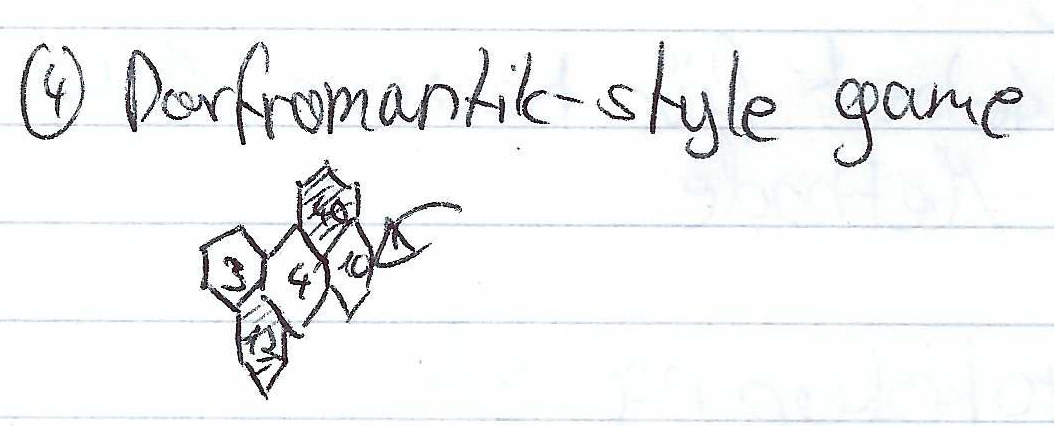
\includegraphics[width=0.5\textwidth]{brainstorming_04_dorfromantik.png}
    \caption{Skizze des \enquote{Dorfromantik}-Ansatzes}
  \end{figure}

  Dieser Ansatz ist inspiriert durch das Videospiel \emph{Dorfromantik}\footnote{\url{https://toukana.com/dorfromantik/}}, in dem verschiedene hexagonale Landschafts-Kacheln auf einem Spielbrett derart angebracht werden müssen, dass sie Synergie-Effekte erzielen.
  Wenn sich das Spielprinzip so anpassen ließe, dass eine Spielerin Kacheln mit verschiedenen Zahlen so platzieren müsste, dass bei der Multiplikation von aneinanderliegenden Kacheln bestimmte Ergebnisse erzielt würden---ähnlich einem Sudoku---so könnte dies eine für Kinder anregende Lernmechanik darstellen.

  \item Kombinationsspiel nach dem Vorbild von 2048
  
  Auch dieser Ansatz zieht Inspiration aus einem Videospiel. Bei \emph{2048}\footnote{\url{https://play2048.co/}} können Spieler Kacheln mit 2er-Potenzen auf einem 4x4-Spielfeld verschieben, wobei zwei aufeinander geschobene Kacheln sich multiplizieren, um eine Kachel mit der Zahl 2048 zu erhalten.
  Um Kindern das Einmaleins beizubringen, könnte dieser Ansatz abgewandelt werden, indem in verschiedenen Spieldurchläufen unterschiedliche Basis-Zahlen als Ausgangskacheln und eine Ziel-Zahl auch dem Einmaleins verwendet würden.

  \item Action-reiches Kombinationsspiel mit Geschick und Zeitdruck
  
  \begin{figure}[h]
    \centering
    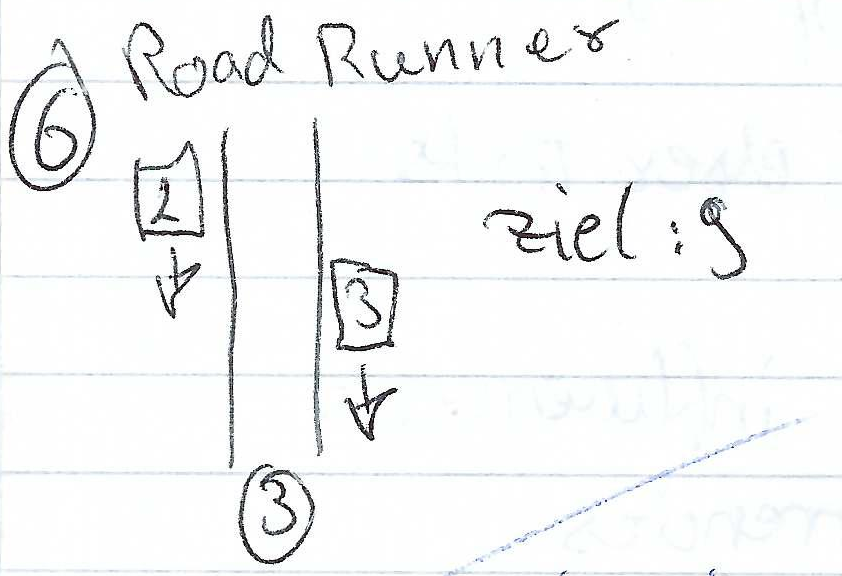
\includegraphics[width=0.5\textwidth]{brainstorming_06_road_runner.png}
    \caption{Skizze des \enquote{Road Runner}-Ansatzes}
  \end{figure}

  Dieser letzte Ansatz soll das Lernen für Kinder interessant gestalten, indem es in eine Herausforderung gegossen wird, welche Geschick und schnelles Denken erfordert.
  Das Spielfeld besteht aus drei senkrechten, parallelen Bahnen auf denen Kacheln mit zufälligen Zahlen am oberen Bildschirmrand auftauchen und sich nach unten bewegen.
  Der Spieler kontrolliert eine weitere Kachel mit einer Zahl, welche er zwischen den Bahnen verschieben kann.
  Wenn eine der \enquote{herunterfallenden} Kacheln die des Spielers trifft, so wird letztere mit ersterer multipliziert und durch das Ergebnis ersetzt.
  Die Aufgabe des Spielers ist es mit seiner Zahl eine vorgegebene zu erreichen.
  Übertritt er das Ziel oder erreicht es nicht in einer Vorgegebenen Zeitspanne, so hat er verloren. 

\end{enumerate}

Die Ansätze 5 und 6 waren beide sehr vielversprechend für mich, aber ich hatte Zweifel, ob es mir möglich sei im Zeitrahmen des Projekts eine zufriedenstellende Spielerfahrung zu implementieren, weswegen ich sie ausgeschlossen habe.
Ähnlich steht es um Ansatz 4. Während ich ihn sehr interessant finde, so war mir doch klar, dass er zu komplex ist, um ihn in in angemessener Zeit zufriedenstellend umzusetzen.
Zudem hatte ich Sorge, dass das Spielprinzip eventuell zu anspruchsvoll für die Zielgruppe von 6--8 Jährigen sein könnte.
Zu Ansatz 3 habe ich mit verschiedenen Analogien, wie den genannten Beispielen, gespielt, aber letztendlich habe ich keine gefunden, bei der ich sicher war, dass sie eine sinnvolle Grundlage für die App darstellen könnte.
Zu guter Letzt blieb mir die Entscheidung zwischen Ansatz 1 und 2, welche mir insofern leicht viel, dass ich beide als ähnlich empfand.
Ich habe Ansatz 1 gewählt, weil ich die Wisch-Mechanik als dynamischer empfand, als das Tippen auf Knöpfe. 
Zudem nahm ich an, dass es bereits eine wiederverwendbare Implementierung von wischbaren Karten gäbe, da die Mechanik durch \emph{Tinder} relativ bekannt ist. 

\section{1 x 1 Mobile-App}

Im Folgenden möchte ich auf die fertige App eingehen. Hierzu gebe ich eine Übersicht der implementierten Features in der Form von User Stories, bevor ich einen Überblick über die Gestaltung der Nutzeroberfläche und der Struktur des Programmcodes gebe.
Dieser Teil schließt mit einer Beschreibung der Test-Routine, welche ich eingesetzt habe, um die korrekte Funktionalität der App zu überprüfen.

\subsection{Features}

Tabelle \ref{tab:features} gibt einen Überblick der Features, welche die App dem Nutzer bietet.

\begin{table}[ht]
  \begin{tabu}{| >{\ttfamily} r | X |}
    \hline
    F1 & Als ein Spieler möchte ich das Einmaleins lernen, indem ich zufällig generierte Multiplikationsgleichungen dadurch in richtig und falsch einordne, dass ich sie nach rechts oder links wische.\\
    \hline
    F2 & Als eine Spielerin möchte ich Punkte für das korrekte Einordnen von Gleichungen sammeln.\\
    \hline
    F3 & Als ein Spieler möchte ich dadurch herausgefordert werden, dass durch das falsche Einordnen von Gleichungen mein Spieldurchlauf beendet werden kann.\\
    \hline
    F4 & Als eine Spielerin möchte ich meine letzte Höchstpunktzahl ansehen können.\\
    \hline
    F5 & Als ein Spieler möchte ich eine Rangliste mit den Höchstpunktzahlen von mir und anderen Spielern ansehen können.\\
    \hline
  \end{tabu}
  \caption{Features der 1 x 1 Mobile-App}\label{tab:features}
\end{table}

\texttt{F1} stellt den Kern der App und dieses Projekt dar.
Es wird durch die \texttt{GamePage} bereitgestellt, welche dem Spieler einen Stapel von wischbaren Karten mit Gleichungen, zusammen mit einem Punktezähler und drei ausgefüllten Herzen, darstellt.
Die Gleichungen werden zufällig generiert, indem zwei Operanden zufällig bestimmt und mit einer 50\% Chance das Ergebnis verfälscht wird.
Wischt der Spieler eine Karte in die richtige Richtung, so wird seinem Punktekonto das Produkt der beiden Operanden gutgeschrieben, wodurch \texttt{F2} erfüllt wird.
Ist die Richtung, in die der Spieler einer Karte wischt, falsch, so wird ihm eines seiner drei Herzen abgezogen.
Hat der Spieler keine Herzen mehr, so ist der Spieldurchlauf beendet und ihm wird die \texttt{GameOverPage} angezeigt.
Dies erfüllt das Feature \texttt{F3}.

\begin{wrapfigure}{l}{0.4\textwidth}
  \centering
  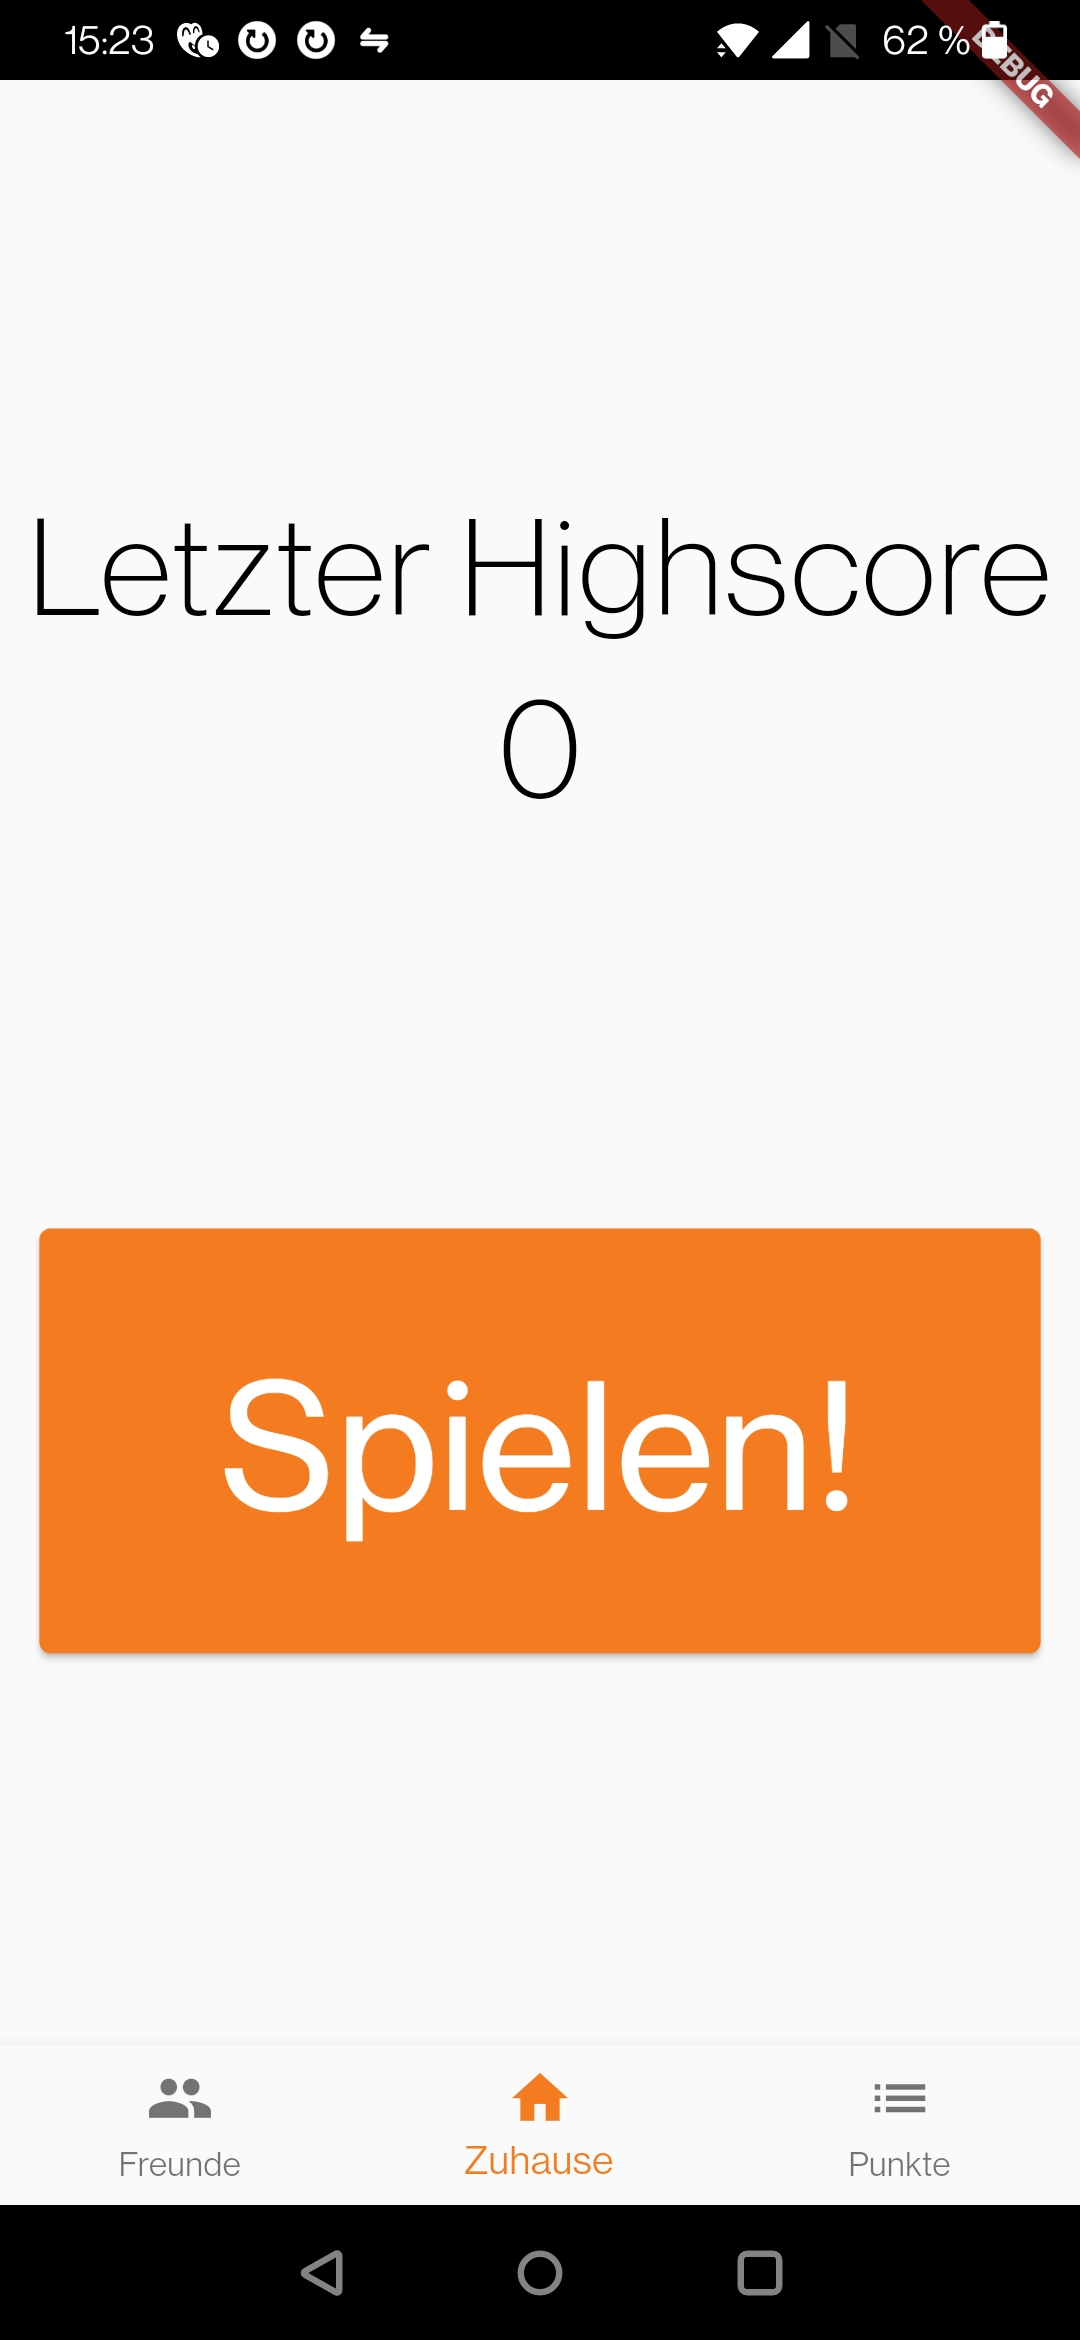
\includegraphics[width=0.35\textwidth]{home_view.jpg}
  \caption{Die \texttt{HomePage}}
\end{wrapfigure}

Das Feature \texttt{F4} wird durch die \texttt{HomePage} bedient, welche immer die von der Spielerin höchste erreichte Punktzahl anzeigt.
Diese Seite bietet zudem noch die \texttt{HighscoreView} Ansicht, die eine Rangliste mit der von der Spieler erreichten Punktzahlen anzeigt und somit Feature \texttt{F5} bedient.
Die notwendigen Netzwerk-Features für das Anzeigen von den Punktzahlen verschiedener Spieler wurden im Rahmen dieses Projektes nicht implementiert.
Zwischen den verschiedenen Ansichten der \texttt{HomePage} kann über eine Navigation am unteren Ende des Bildschirms gewechselt werden.

Das Speichern der Punktzahlen setzt eine lokale Persistenz für die Daten der App voraus, welche mittels des \emph{flutter}-Pakets \emph{sqflite} implementiert wurde.
Diese Bibliothek bietet Funktionalitäten um Daten in einer auf dem lokalen Dateisystem abgelegte SQLite-Datenbank zu verwalten.
Ein Problem, welches durch die Verwendung von \emph{sqflite} aufkam, ist, dass die Datenbank nach dem Starten der App zunächst initialisiert werden muss.
Dies geschieht asynchron, jedoch muss dem Spieler für die Dauer der Initialisierung eine Übergangsansicht angezeigt werden, da man ihm keine Ansicht ohne Daten anzeigen möchte.

Aus diesem Grund ist die initiale Ansicht der App die \texttt{SplashPage}, welche für die Dauer der Initialisierung einen Ladeindikator anzeigt.
Nach dem Abschluss der Initialisierung leitet sie den entweder auf die \texttt{HomePage} oder die \texttt{LandingPage} weiter, sollten noch keine Daten in der Datenbank vorliegen.
Auf der \texttt{LandingPage} kann der Nutzer seinen Namen eintragen, bevor er zur \texttt{HomePage} weitergeleitet wird.

\begin{figure}[h]
  \centering
  \begin{subfigure}[b]{0.4\textwidth}
    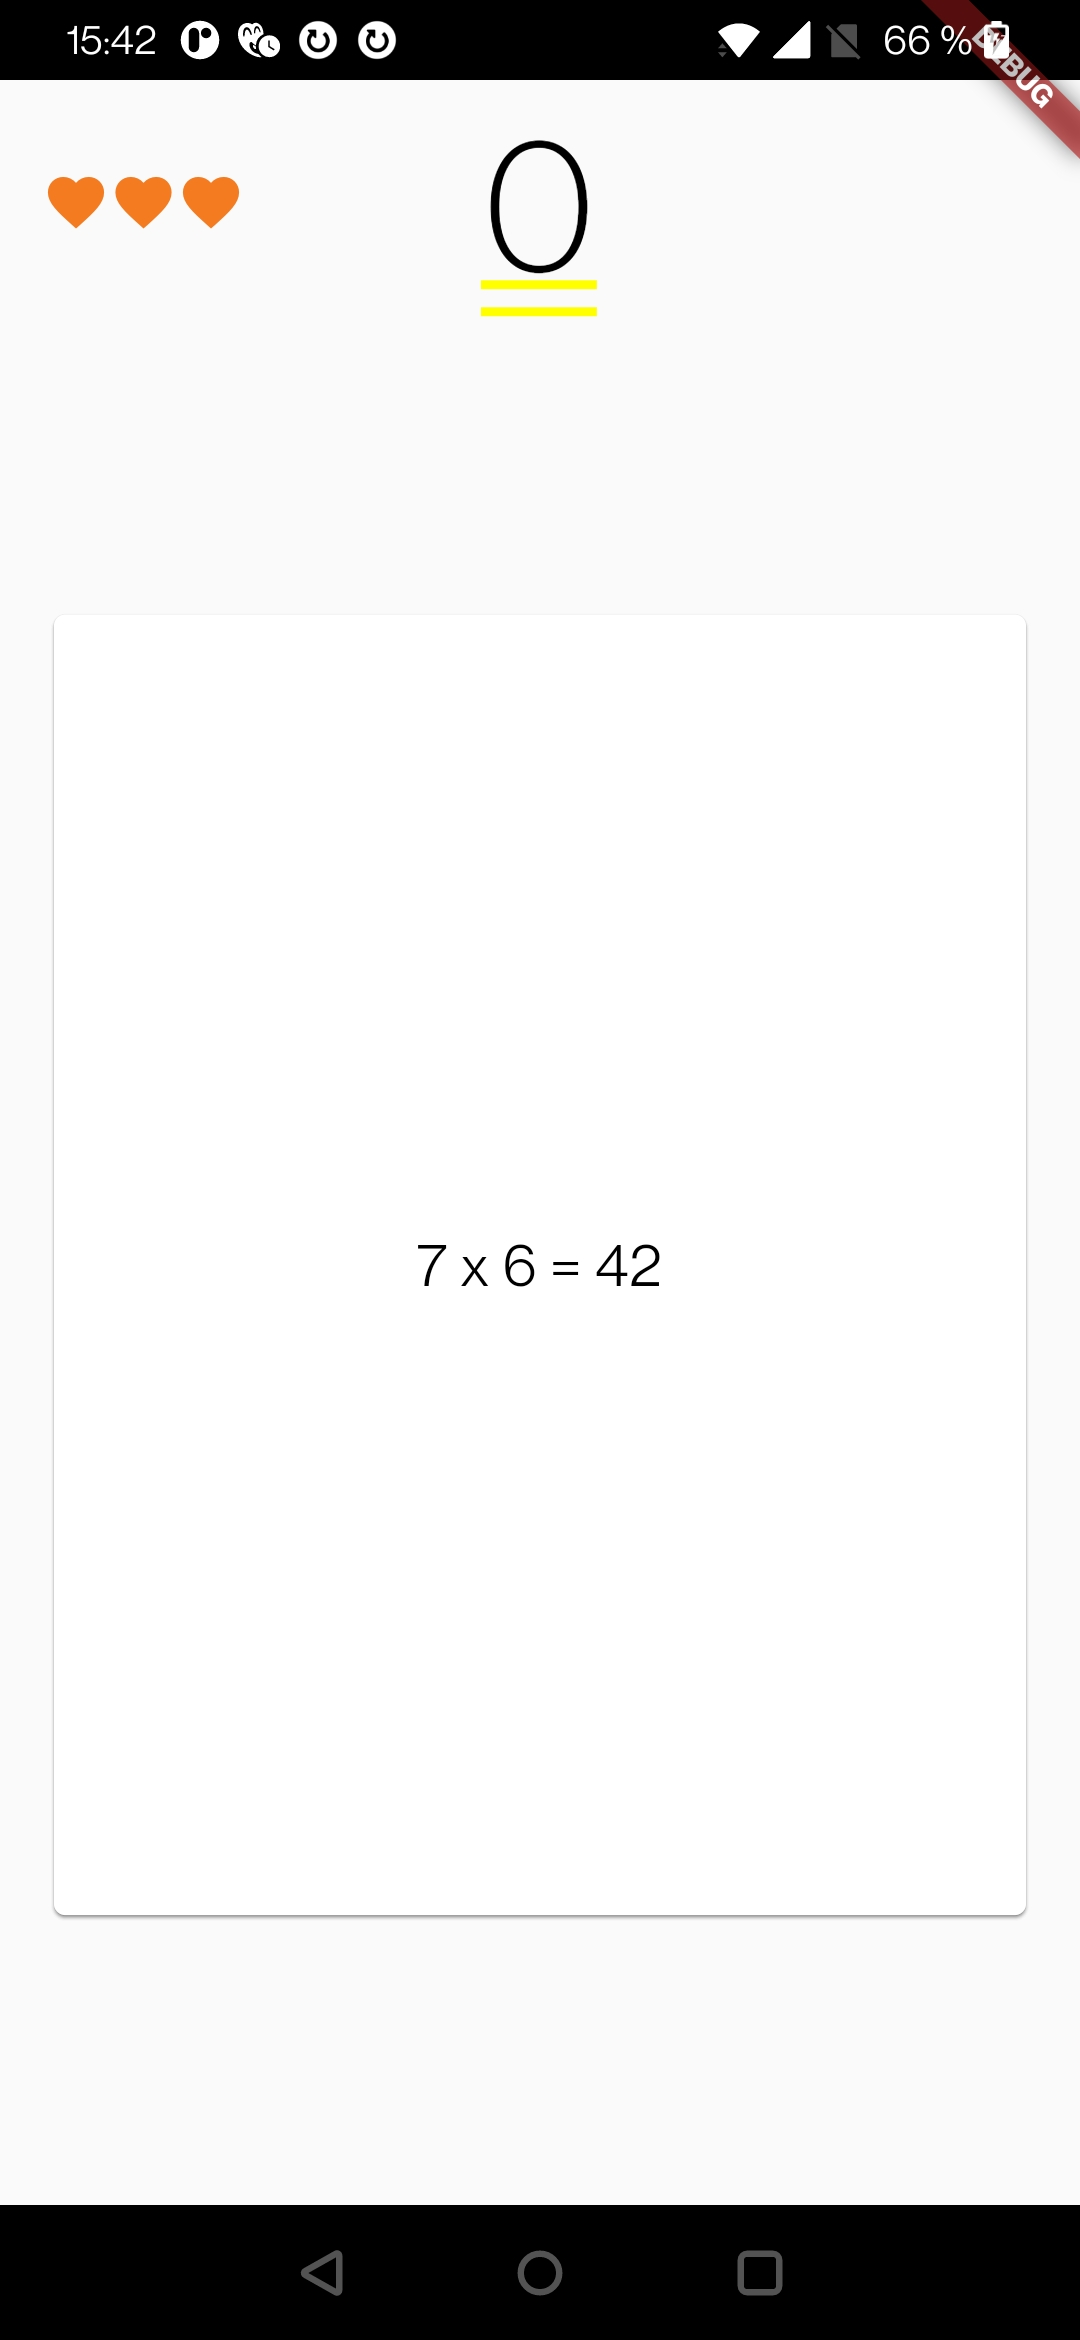
\includegraphics[width=\textwidth]{game_view.jpg}
    \caption{Die \texttt{GamePage}}
  \end{subfigure}
  ~
  \begin{subfigure}[b]{0.4\textwidth}
    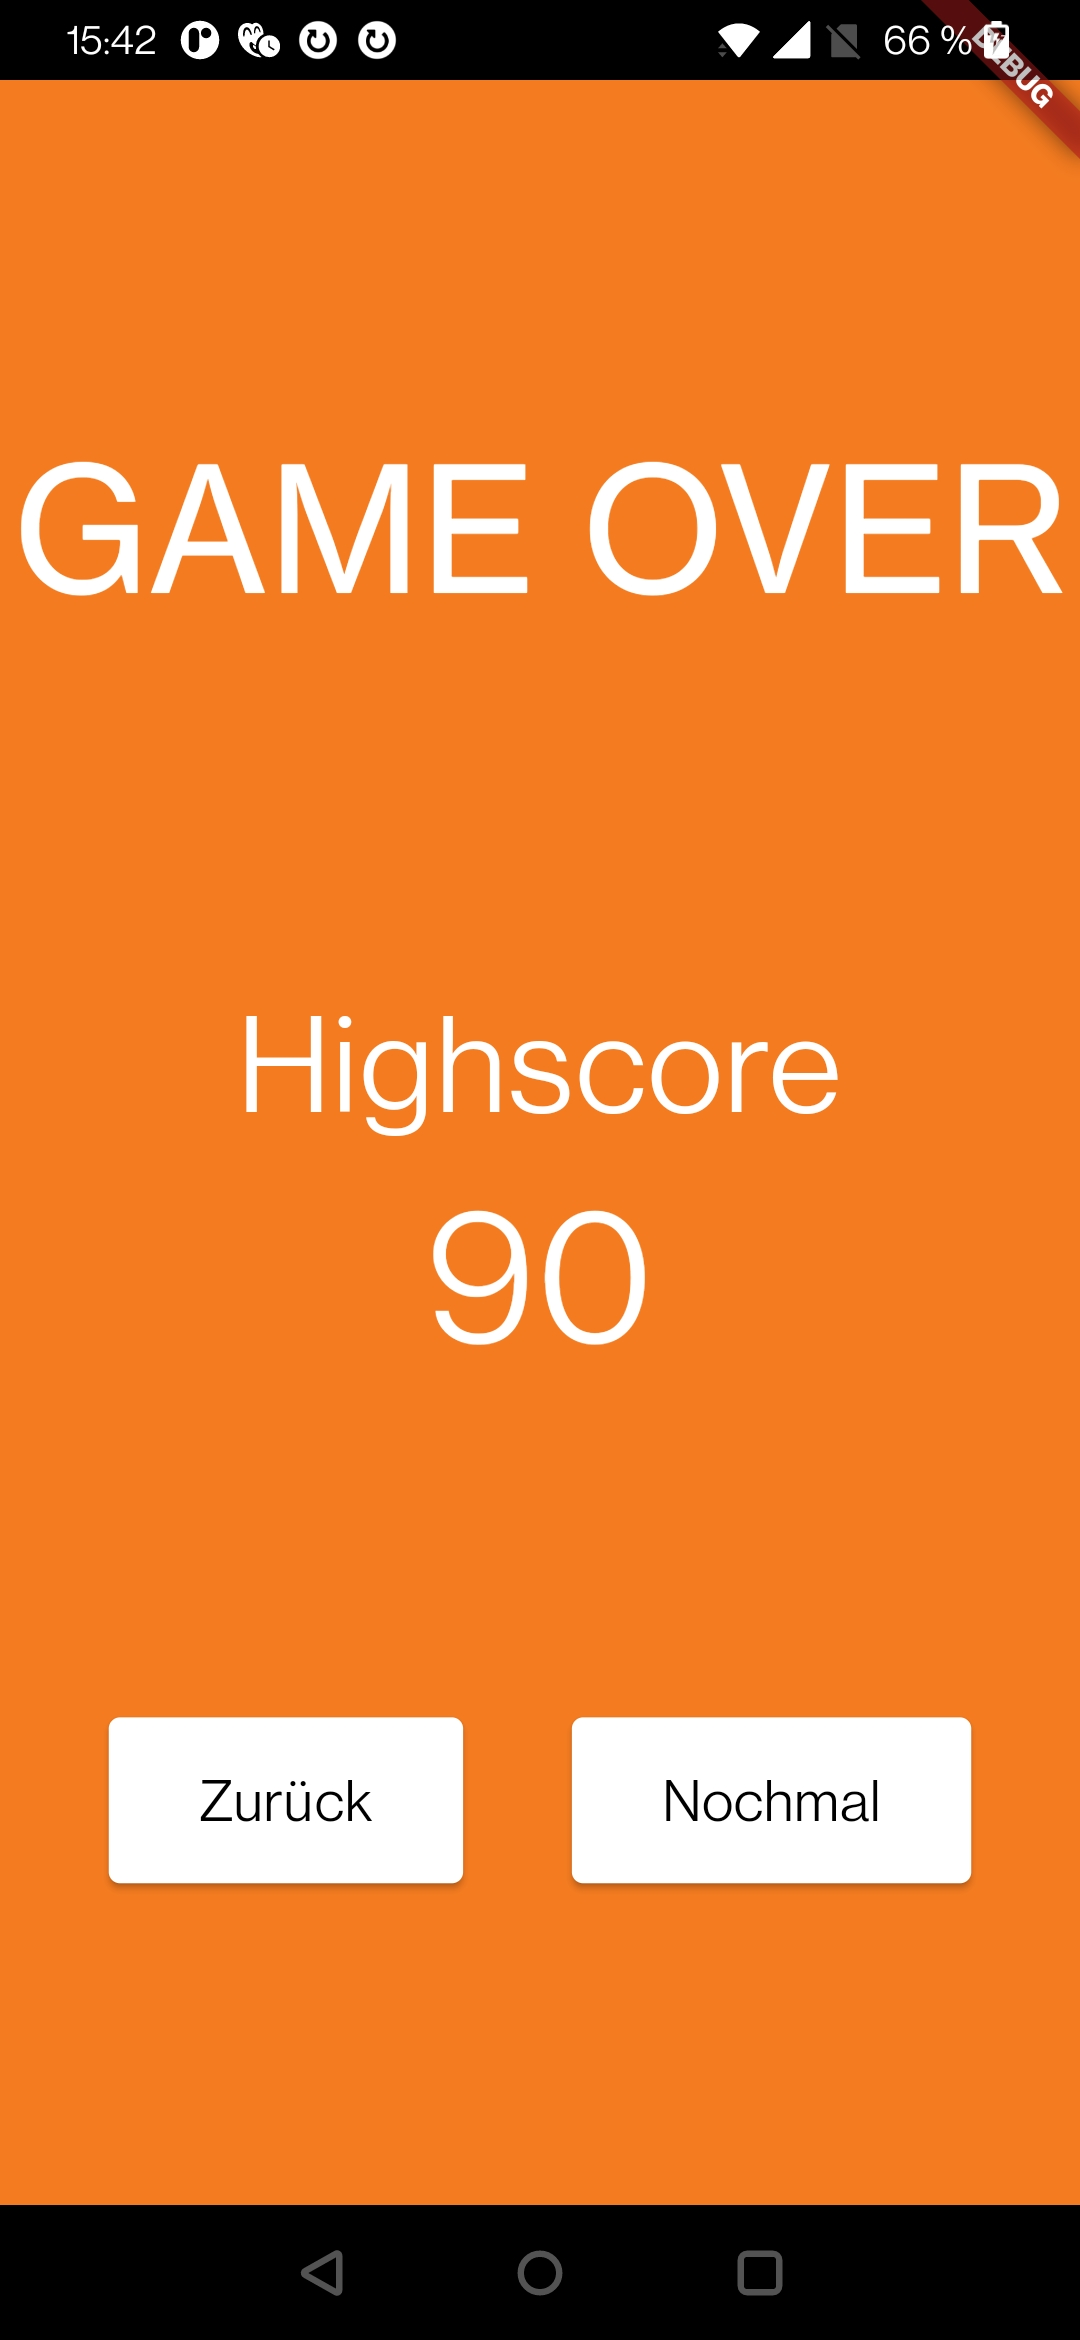
\includegraphics[width=\textwidth]{game_over_view.jpg}
    \caption{Die \texttt{GameOverPage}}
  \end{subfigure}
\end{figure}

\subsection{Design}

Das Design der App sollte zugleich simpel und ansprechend sein, weswegen einfaches Schwarz und Weiß als Grund- und ein freundliches Orange als Kontrastfarben gewählt wurden.
Gleichzeitig sollte das Design möglichst plattformunabhängig sein, da \emph{flutter}-Apps besonders einfach auf sowohl iOS wie auch Android auszuliefern sind.
Abgerundete Knöpfe und eine leichte Schriftart sollen ebenfalls zu dem ansprechenden Design beitragen.

\subsection{Struktur}

In diesem Abschnitt gehe ich auf die Struktur des Programmcodes des Mobile-App ein.
Grundsätzlich bin ich nicht strikt den Paradigmen der objektorientierten Programmierung, sondern habe einen Mix aus Klassen, Konstanten und Funktionen gewählt.

Die folgende Auflistung stellt die Ordnerstruktur des \texttt{lib}-Ordners des Projekts dar und gibt kurze Erläuterungen zu dem Inhalt der einzelnen Unterordner.
Da die Ordnerstruktur in \emph{flutter}'s Programmiersprache \emph{Dart} ebenfalls die Paketstruktur des Programms darstellt, ist dies zugleich eine Darstellung der logischen Struktur des Codes.

 \begin{itemize}
   \item \texttt{infrastructure}
   
    Dieses Paket enthält verschiedene Artefakte, welche die grundlegende Infrastruktur des Programms bereitstellen und verwalten.
    Konkret finden sich hier aktuell nur ein globales Objekt für den Datenbankzugriff und etwas Code zur Initialisierung der Datenbank.

   \item \texttt{model}
   
    Hier finden sich Artefakte, die Domänen-Entitäten modellieren.
    Die hier definierten Klassen dienen dem Datenaustausch zwischen den Komponenten des Programms.

   \item \texttt{repository}
   
    Dieses Paket bietet verschiedene \emph{Repositories} an, welche den Datenbankzugriff auf ihre jeweiligen Domänen-Entitäten verschalen.

   \item \texttt{theme}
   
    Das \texttt{theme} Paket enthält verschiedene Konstanten, welche den visuellen Stil der Anwendung bestimmen, wie zum Beispiel Farben oder Schriftarten.
    Auf diese Art sind diese Informationen gebündelt und können zentral verändert werden.

   \item \texttt{ui}
   
    Dieses Paket ist das wohl umfangreichste, denn hier sind sämtliche Elemente der Benutzeroberfläche definiert.
   
   \begin{itemize}
     \item \texttt{component}
     
      Hier finden sich alle Komponenten, welche entweder in mehreren Ansichten verwendet werden oder die schlicht zu umfangreich sind um in der Definition der Ansicht zu stehen, welche sie verwendet.
      Auf die beiden Komponenten, die aktuell hier definiert sind, trifft letzteres zu. 

     \item \texttt{page}
     
     Dieses Paket enthält alle Ansichten der App.
     Sollte eine Ansicht mehrere Unteransichten haben---wie die \texttt{HomePage}---so finden sich diese in weiter verschachtelten Paketen.
   \end{itemize}
 \end{itemize}

\subsection{Tests}

Aufgrund des geringen Umfang und begrenzten Zeitraumes des Projekts habe ich mich dagegen entschieden klassische Unit Tests für die einzelnen Komponenten der App zu schreiben.
Stattdessen habe ich für jedes Feature eine einfache Testroutine definiert, welche ich manuell durchgehen konnte um die korrekte Funktionsweise des Features sicherzustellen.
Tabelle \ref{tab:test-routines} zeigt eine Aufstellung dieser Testroutinen.

\begin{table}
  \begin{longtabu}{| >{\ttfamily} r | X |}
    \hline
    F1.1 & Bei uninitialisierter App. Wenn ich als Spieler die App öffne wird mir kurz die \texttt{SplashPage} angezeigt und dann werden ich zur \texttt{LandingPage} navigiert. \\
    \hline
    F1.2 & Wenn ich als Spieler auf der \texttt{LandingPage} meinen Namen eingebe und die Eingabe bestätige, dann werden ich auf die \texttt{HomePage} navigiert. \\
    \hline
    F1.3 & Bei initialisierter App. Wenn ich als Spieler die App öffne wird mir kurz die \texttt{SplashPage} angezeigt und dann werden ich zur \texttt{HomePage} navigiert. \\
    \hline
    F1.4 & Wenn ich als Spieler auf der \texttt{HomePage} den \enquote{Spielen!}-Knopf drücke, werde ich zur \texttt{GamePage} navigiert.\\
    \hline
    F1.5 & Ich als Spieler kann auf der \texttt{GamePage} Karten mit Gleichungen nach rechts oder links wischen und sie verschwinden.\\
    \hline
    F2.1 & Wenn ich als Spielerin eine korrekte Gleichung nach rechts wische, erhalte ich das Ergebnis der Gleichung zu meiner Punktzahl hinzu.\\
    \hline
    F2.2 & Wenn ich als Spielerin eine inkorrekte Gleichung nach links wische, erhalte ich das Produkt der Operanden zu meiner Punktzahl hinzu.\\
    \hline
    F3.1 & Wenn ich als Spieler eine korrekte Gleichung nach links wische oder eine inkorrekte Gleichung nach rechts wische, erlischt eines meiner Herzen.\\
    \hline
    F3.2 & Wenn ich als Spieler keine Herzen mehr habe, werde ich zur \texttt{GameOverPage} navigiert.\\
    \hline
    F3.3 & Wenn ich als Spieler auf der \texttt{GameOverPage} auf den \enquote{Zurück}-Knopf drücke, werde ich zur \texttt{HomePage} navigiert.\\
    \hline
    F3.4 & Wenn ich als Spieler auf der \texttt{GameOverPage} auf den \enquote{Nochmal}-Knopf drücke, werde ich auf die \texttt{GamePage} navigiert. Die \texttt{GamePage} ist im initialen Zustand.\\
    \hline
    F4.1 & Mir als Spielerin wird auf der \texttt{HomePage} meine höchste erreichte Punktzahl angezeigt.\\
    \hline
    F5.1 & Wenn ich als Spieler auf den \enquote{Punkte}-Knopf drücke, werde ich zur \texttt{HighscoreView} navigiert. Die \texttt{HighscoreView} zeigt alle meine vergangenen Punktestände in absteigender Reihenfolge zusammen mit meinem Namen an.\\
    \hline
  \end{longtabu}
  \caption{Testroutinen für alle Features}\label{tab:test-routines}
\end{table}

Es ist anzumerken, dass sich zum Ende des Projektes immer noch ein Fehler im Programm befindet, welcher ab und zu scheinbar zufällig auftritt und verhindert, dass gewischte Karten auf der \texttt{GamePage} auch verschwinden.
Sollte dieser Fehler auftreten, so muss der Spieldurchlauf durch eine Rückwärtsnavigation und erneutes Drücken auf \enquote{Spielen!} neu gestartet werden.

\section{Schluss}

Zum Abschluss möchte ich noch einmal kurz den bisherigen Text zusammenfassen und einen Ausblick darüber geben, welche Weiterentwicklung für die App möglich wären, würde das Projekt weitergeführt.

In dieser Dokumentation habe ich den Prozess beschrieben mit dem ich zur Grundlegenden Idee für das Konzept der App gekommen bin und habe einige interessante Alternativen beschrieben, welche ich zugunsten des \enquote{Tinder}-Ansatzes nicht verfolgt habe.
Anschließend folgte eine Darlegung der konkreten Features der App, ihrer visuellen Design-Philosophie und der Struktur ihres Programmcodes.
Zuletzt habe ich dargestellt, wie ich die korrekte Funktionsweise der App mittels manuellen Testroutinen überprüft habe.

Gerne hätte ich die App im Rahmen des Projektes um noch mehr Funktionalität und Elemente der Gamification erweitert.
Besonders fehlen mir audiovisuelles Feedback und soziale Elemente.
Darüber hinaus wären auch ein Modus mit Zeitlimit für das Einordnen von Gleichungen für eine größere Herausforderung und ein progressiv ansteigender Schwierigkeitsgrad denkbar.

Auch einige der anderen vorgestellten Ansätze für solch eine Lern-App hätte ich gerne verfolgt.
Besonders den \enquote{Dorfromantik}- und den \enquote{Road Runner}-Ansatz.

Hauptsächlich jedoch freue ich mich darüber das \emph{flutter} Framework nach meinem lange zurückliegenden Erstkontakt auf diese Art und Weise noch einmal im Detail kennen lernen zu können.
